\chapter{Polarizações de ondas massivas: o TG revisitado}
\label{cap:polarizacoes}

Este capítulo refaz o cálculo central do TG sem a hipótese de
propagação quase nula. A estratégia é trabalhar diretamente com a matriz
de marés $E_{ij}$. Ela é o observável local, não depende do calibre e
não exige a escolha de uma tétrada. Os resultados são de três tipos. O
primeiro confirma a contagem de seis amplitudes independentes no modelo
de Visser e explica a origem da sexta. O segundo contrasta esse modelo
com Fierz--Pauli. O terceiro delimita o domínio de validade das
expressões NP e das classes E(2) usadas no TG, e reavalia a comparação
entre bandas de frequência. Todas as identidades algébricas deste
capítulo foram verificadas simbolicamente
(Apêndice~\ref{ap:reproducao}).

\section{Convenções}

Usam-se $c=1$ e a assinatura $(+,-,-,-)$. Uma onda plana que se propaga
ao longo de $+z$ é escrita como
\begin{equation}
 g_{\mu\nu}=\eta_{\mu\nu}+\operatorname{Re}\left[H_{\mu\nu}\,
 e^{-i\omega t+ikz}\right],
 \qquad \omega>0,\quad k\geq0,
 \label{eq:pol-onda}
\end{equation}
com amplitudes $H_{\mu\nu}$ constantes e possivelmente complexas.
Definem-se
\begin{equation}
 \Delta=\omega^2-k^2,\qquad \Sigma=\omega^2+k^2,\qquad
 \beta=\frac{k}{\omega},\qquad
 \chi=1-\beta^2=\frac{\Delta}{\omega^2}.
 \label{eq:pol-defs}
\end{equation}
Nas teorias massivas consideradas, a relação de dispersão é
$\Delta=\mu^2$, com $\mu=m_gc/\hbar$. Em unidades físicas,
\begin{equation}
 \beta=\frac{v_g}{c}=\sqrt{1-\left(\frac{f_g}{f}\right)^2},
 \qquad \chi=\left(\frac{f_g}{f}\right)^2,
 \qquad f_g=\frac{m_gc^2}{h}.
 \label{eq:pol-dispersao}
\end{equation}
O parâmetro $\epsilon$ da Eq.~\eqref{eq:fund-epsilon}, usado no TG,
relaciona-se a essas grandezas por $\epsilon=1/\beta^2-1=\chi/\beta^2$.
Ondas viajantes exigem $f>f_g$. O ponto $f=f_g$ ($k=0$) é o
\emph{limiar}: nele, a onda é espacialmente homogênea.

A massa é sempre definida pela relação de dispersão. A
Seção~\ref{sec:pol-normalizacao} mostra por que essa escolha é necessária
ao comparar com o TG e o artigo de 2004.

\section{Matriz de marés sem hipótese de nulidade}

O Riemann linearizado é
\begin{equation}
 R_{\alpha\beta\gamma\delta}=\frac12\left(
 H_{\alpha\delta,\beta\gamma}+H_{\beta\gamma,\alpha\delta}
 -H_{\alpha\gamma,\beta\delta}-H_{\beta\delta,\alpha\gamma}\right).
 \label{eq:pol-riemann}
\end{equation}
Para a onda plana, cada par de derivadas introduz $-q_\mu q_\nu$, com
$q_\mu=(-\omega,0,0,k)$. As seis componentes de $E_{ij}=R_{0i0j}$ são
\begin{equation}
 \begin{aligned}
 E_{11}&=\tfrac12\omega^2H_{11}, &
 E_{22}&=\tfrac12\omega^2H_{22}, &
 E_{12}&=\tfrac12\omega^2H_{12},\\
 E_{13}&=\tfrac12\omega\,(\omega H_{13}+kH_{01}), &
 E_{23}&=\tfrac12\omega\,(\omega H_{23}+kH_{02}), &
 E_{33}&=\tfrac12\left(\omega^2H_{33}+2\omega kH_{03}+k^2H_{00}\right).
 \end{aligned}
 \label{eq:pol-mares-geral}
\end{equation}
Até aqui não se usou equação de campo, calibre ou relação de dispersão.
A Eq.~\eqref{eq:pol-mares-geral} vale para qualquer teoria métrica
linearizada em torno de Minkowski. Para descrever as deformações,
usam-se as seis coordenadas
\begin{equation}
 \mathbf p=(p_b,\,p_l,\,p_+,\,p_\times,\,p_x,\,p_y)
 =(E_{11}+E_{22},\;E_{33},\;E_{11}-E_{22},\;E_{12},\;E_{13},\;E_{23}),
 \label{eq:pol-coordenadas}
\end{equation}
correspondentes aos modos \emph{breathing}, longitudinal, $+$, $\times$
e aos dois vetoriais.

O apêndice em Maple do TG usa a convenção oposta de sinal do Riemann:
por exemplo, o TG obtém $R_{txtx}=-\frac12A_{11}\omega^2$, enquanto a
Eq.~\eqref{eq:pol-mares-geral} dá $+\frac12\omega^2H_{11}$. Trata-se de
uma inversão global, $R^{\rm TG}=-R$. Ela não altera contagens nem
razões entre componentes, mas deve ser acompanhada ao combinar as
expressões do TG com a equação do desvio geodésico.

\section{O modelo linear de Visser: seis amplitudes}

No modelo de Visser linearizado, as equações de campo implicam
\begin{equation}
 q^\mu\bar H_{\mu\nu}=0
 \label{eq:pol-vinculo-visser}
\end{equation}
e $(\Box+\mu^2)\bar H_{\mu\nu}=0$, isto é, $\Delta=\mu^2$
(Seção~\ref{sec:fund-massiva}; TG, eqs.~4.14 e 4.20). A condição
\eqref{eq:pol-vinculo-visser} tem a forma da condição harmônica da RG,
mas aqui ela é um vínculo das equações, não uma escolha de calibre. Uma
transformação $H_{\mu\nu}\to H_{\mu\nu}+q_\mu\xi_\nu+q_\nu\xi_\mu$ muda
o lado esquerdo por $\Delta\,\xi_\nu$ e, portanto, não preserva o
vínculo quando $\Delta\neq0$. Não há como eliminar modos por calibre
na teoria massiva.

As quatro equações \eqref{eq:pol-vinculo-visser} podem ser resolvidas
para $(H_{01},H_{02},H_{03},H_{11})$ em termos de seis amplitudes
livres, que se escolhem como
$(A,D,B,C,V_x,V_y)=(H_{00},H_{33},H_{22},H_{12},H_{13},H_{23})$:
\begin{equation}
 H_{01}=-\frac{k}{\omega}V_x,\quad
 H_{02}=-\frac{k}{\omega}V_y,\quad
 H_{03}=-\frac{\omega k}{\Sigma}(A+D),\quad
 H_{11}=-B-\frac{\Delta}{\Sigma}(A+D).
 \label{eq:pol-solucao-visser}
\end{equation}
Não houve divisão por $k$ nem por $\Delta$: a parametrização é regular
no limiar e no caso nulo. Substituindo em
\eqref{eq:pol-mares-geral},
\begin{equation}
 E^{\rm V}=\frac12
 \begin{pmatrix}
 -\omega^2\!\left(B+\dfrac{\Delta}{\Sigma}(A+D)\right) & \omega^2C & \Delta V_x\\[2mm]
 \omega^2C & \omega^2B & \Delta V_y\\[1mm]
 \Delta V_x & \Delta V_y & \dfrac{\Delta}{\Sigma}(\omega^2D-k^2A)
 \end{pmatrix}.
 \label{eq:pol-mares-visser}
\end{equation}
O jacobiano do mapa $(A,D,B,C,V_x,V_y)\mapsto\mathbf p$ é
\begin{equation}
 \det\frac{\partial\mathbf p}{\partial(A,D,B,C,V_x,V_y)}
 =\frac{\omega^6\Delta^4}{32\,\Sigma}.
 \label{eq:pol-det-visser}
\end{equation}
Para qualquer onda massiva ($\Delta\neq0$), inclusive no limiar, o
determinante é não nulo.

\paragraph{Resultado 1.} \emph{No modelo linear de Visser, as seis
componentes da matriz de marés são amplitudes independentes. A contagem
de seis polarizações do TG está correta.} Essa conclusão é exata em
$f/f_g$ e coincide com as amplitudes exatas obtidas por Hyun, Kim e Lee
\autocite{hyun2019}, após tradução de assinatura e ordenação.

\section{Fierz--Pauli: cinco amplitudes e um vínculo escalar}

Em Fierz--Pauli ($a=1$ na Eq.~\ref{eq:fund-familia}), as equações
implicam
\begin{equation}
 H=0,\qquad q^\mu H_{\mu\nu}=0,\qquad \Delta=\mu^2.
 \label{eq:pol-vinculos-fp}
\end{equation}
Com traço nulo, os vínculos de Visser e de Fierz--Pauli coincidem. A
diferença entre as teorias é, portanto, exatamente a condição $H=0$.
Na parametrização \eqref{eq:pol-solucao-visser}, o traço vale
\begin{equation}
 H=\frac{2\left(\omega^2A-k^2D\right)}{\Sigma},
 \label{eq:pol-traco}
\end{equation}
e $H=0$ impõe $A=k^2D/\omega^2$. A matriz de marés fica
\begin{equation}
 E^{\rm FP}=\frac12
 \begin{pmatrix}
 -\omega^2B-\Delta D & \omega^2C & \Delta V_x\\
 \omega^2C & \omega^2B & \Delta V_y\\
 \Delta V_x & \Delta V_y & \Delta^2D/\omega^2
 \end{pmatrix},
 \label{eq:pol-mares-fp}
\end{equation}
com cinco amplitudes, e o mapa para $(p_b,p_+,p_\times,p_x,p_y)$ tem
determinante $\omega^4\Delta^3/16\neq0$. As duas deformações escalares
não são mais independentes:
\begin{equation}
 p_b=-\frac{\Delta D}{2},\qquad
 p_l=\frac{\Delta^2D}{2\omega^2}
 \qquad\Longrightarrow\qquad
 \boxed{\;p_l=-\left(\frac{f_g}{f}\right)^2p_b\;}
 \label{eq:pol-vinculo-escalar}
\end{equation}
Em Fierz--Pauli, os modos \emph{breathing} e longitudinal são duas
manifestações da mesma amplitude de helicidade zero. Longe do limiar, o
modo escalar aparece quase só como \emph{breathing}; no limiar,
$p_l=-p_b$ e a maré escalar não tem traço.

\paragraph{Resultado 2.} \emph{O sexto modo do modelo de Visser é o
traço da perturbação.} Em Visser, as deformações escalares são livres,
e seu desvio do vínculo \eqref{eq:pol-vinculo-escalar} é proporcional
ao traço:
\begin{equation}
 p_l+\left(\frac{f_g}{f}\right)^2p_b=-\frac{\Delta}{4}\,H .
 \label{eq:pol-identidade-traco}
\end{equation}
O traço é justamente o escalar que, em teorias lineares não
Fierz--Pauli, tem energia cinética de sinal errado
(Seção~\ref{sec:fund-fantasma}). Combinando os dois fatos, a interpretação física do
TG fica clara. Das seis polarizações do modelo de Visser, cinco são as
de um gráviton massivo de spin dois; a sexta é um fantasma escalar, de
mesma massa. Esse fantasma permite ao modelo evitar a descontinuidade
vDVZ na ordem linear. Observacionalmente, a
Eq.~\eqref{eq:pol-identidade-traco} diz como distinguir as duas teorias:
em Fierz--Pauli, a razão entre as deformações longitudinal e
\emph{breathing} é fixada pela frequência; no modelo de Visser, não.

\subsection{A polarização de helicidade zero}

Impondo ainda $C=V_x=V_y=0$ e $E_{11}=E_{22}$ em
\eqref{eq:pol-mares-fp}, isola-se a helicidade zero. É conveniente
normalizá-la como as polarizações tensoriais. Sejam $e^1,e^2$ vetores
unitários transversais, $\hat\Omega$ a direção de propagação e
\begin{equation}
 U_\mu=\frac{(\beta,-\hat\Omega)}{\sqrt\chi},
 \qquad U_\mu U^\mu=-1.
 \label{eq:pol-U}
\end{equation}
A polarização
\begin{equation}
 \epsilon^{(0)}_{\mu\nu}=\frac{e^1_\mu e^1_\nu+e^2_\mu e^2_\nu
 -2U_\mu U_\nu}{\sqrt3}
 \label{eq:pol-helicidade-zero}
\end{equation}
é transversa ($q^\mu\epsilon^{(0)}_{\mu\nu}=0$), sem traço e tem a mesma
norma de Lorentz das polarizações $+$ e $\times$,
$\epsilon^{(0)}_{\mu\nu}\epsilon^{(0)\mu\nu}=2$. Para
$H_{\mu\nu}=h_0\,\epsilon^{(0)}_{\mu\nu}$, a matriz de marés é
\begin{equation}
 E^{(0)}=\frac{\omega^2h_0}{2\sqrt3}\,
 \operatorname{diag}\left(1,\;1,\;-2\chi\right).
 \label{eq:pol-mares-h0}
\end{equation}
Duas propriedades dessa expressão serão usadas adiante. A parte
transversal da maré não é suprimida quando $f\gg f_g$; apenas a
longitudinal é. Além disso, algumas componentes métricas de
$\epsilon^{(0)}$ crescem como $1/\chi$: por exemplo,
$\epsilon^{(0)}_{00}=-2\beta^2/(\sqrt3\chi)$. A maré permanece finita
porque essas componentes grandes se cancelam no Riemann.

\section{O ponto de vista da normalização: quão ``pequenos'' são os modos adicionais?}
\label{sec:pol-escala}

O TG e o artigo de 2004 compararam as amplitudes NP em várias
frequências supondo \emph{componentes métricas comparáveis},
$|H_{\mu\nu}|\sim h$ \autocite{tg2003,depaula2004}. Com essa hipótese, a
Eq.~\eqref{eq:pol-mares-visser} mostra que as marés tensoriais escalam
com $\omega^2h$, enquanto todas as não tensoriais escalam com
$\Delta h=\mu^2h$, independentemente da frequência. A razão entre elas
é, portanto,
\begin{equation}
 \frac{|E_{\rm não\ tensorial}|}{|E_{\rm tensorial}|}\sim
 \frac{\Delta}{\omega^2}=\left(\frac{f_g}{f}\right)^2
 \qquad (|H_{\mu\nu}|\sim h).
 \label{eq:pol-supressao}
\end{equation}
Esse é o conteúdo exato da comparação do TG. Os números do artigo de
2004 seguem essa lei: com $f_g\simeq1{,}06\times10^{-7}\,\mathrm{Hz}$,
as razões entre as partes tensorial e massiva de $\Psi_4$ ali
reportadas, $\sim10^{18}$ em $100\,\mathrm{Hz}$ e $\sim10^8$ em
$10^{-3}\,\mathrm{Hz}$, seguem, a menos de fatores numéricos de ordem
um, os valores $(f/f_g)^2\simeq9\times10^{17}$ e $9\times10^7$
\autocite{depaula2004}.

A Figura~\ref{fig:pol-supressao} atualiza essa comparação com os limites
da Tabela~\ref{tab:fund-limites}. Com
$m_g\lesssim2\times10^{-23}\,\mathrm{eV}/c^2$, a razão é menor que
$10^{-18}$ na banda dos interferômetros terrestres e da ordem de
$10^{-9}$ ou menor na do LISA. Ela só atinge a ordem da unidade na banda das
PTAs.

\begin{figure}[htbp]
 \centering
 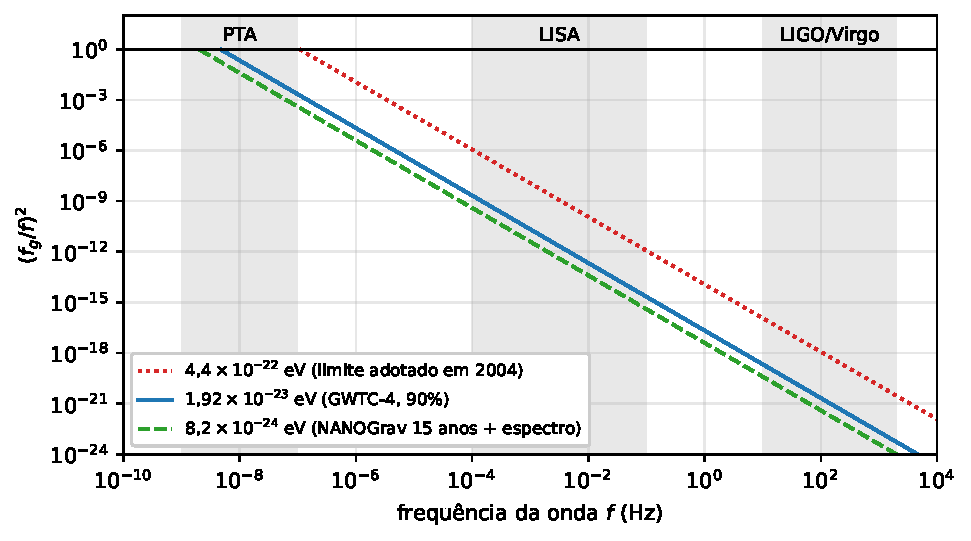
\includegraphics[width=.92\textwidth]{../figuras/supressao.pdf}
 \caption{Razão $(f_g/f)^2$ entre marés não tensoriais e tensoriais
 para componentes métricas comparáveis, Eq.~\eqref{eq:pol-supressao},
 para o limite adotado em 2004 e para dois limites atuais. As curvas
 terminam em $f=f_g$, abaixo do qual não há ondas viajantes. As faixas
 cinzas indicam as bandas aproximadas de PTAs, LISA e interferômetros
 terrestres.}
 \label{fig:pol-supressao}
\end{figure}

Essa conclusão, porém, depende de uma escolha de normalização que a
cinemática não fixa. Se a helicidade zero for normalizada como na
Eq.~\eqref{eq:pol-helicidade-zero}, isto é, com a mesma norma dos modos
tensoriais, a Eq.~\eqref{eq:pol-mares-h0} mostra que sua maré
transversal é da mesma ordem da tensorial em qualquer frequência. Só a
componente longitudinal é suprimida por $(f_g/f)^2$. Para produzir essa
maré, as componentes métricas precisam ser da ordem de $h_0/\chi$. Com
a hipótese $|H_{\mu\nu}|\sim h$, a amplitude de helicidade zero fica,
portanto, implicitamente suprimida por um fator $\chi$.

Qual normalização é fisicamente relevante depende de quanta energia as
fontes irradiam em cada helicidade. Isso não é uma questão de
propagação. É a mesma questão da descontinuidade vDVZ: em Fierz--Pauli
linear, a helicidade zero não se desacopla das fontes quando
$m_g\to0$. Em teorias não lineares, sua emissão perto das fontes é
controlada pelo mecanismo de Vainshtein (Seção~\ref{sec:fund-naolinear}). Duas afirmações
são, portanto, robustas e independem da normalização:
\begin{enumerate}
 \item as assinaturas \emph{especificamente massivas} são suprimidas por
 potências de $f_g/f$. Isso inclui o atraso de propagação
 ($1-\beta\simeq\chi/2$), a componente longitudinal e o vínculo
 \eqref{eq:pol-vinculo-escalar} entre as deformações escalares. Com os
 limites atuais, elas só são de ordem um na banda das PTAs;
 \item em frequências $f\gg f_g$, uma helicidade zero eventualmente
 emitida se manifestaria como um modo \emph{breathing} puro,
 indistinguível, pela forma da maré, do modo escalar de uma teoria
 escalar--tensorial.
\end{enumerate}
A conclusão do TG de que detectores de baixa frequência são os mais
adequados sobrevive nessa forma mais precisa. Nos Capítulos~\ref{cap:pta}
e~\ref{cap:simulacoes}, a potência da helicidade zero é tratada como um
parâmetro livre, justamente porque a cinemática não a fixa.

\section{Validade do formalismo NP e das classes E(2)}

\subsection{O grupo de estabilidade de uma onda massiva}
\label{sec:pol-grupo}

A classificação E(2) usa as transformações de Lorentz que preservam o
vetor de onda. Para uma onda nula, esse grupo é isomorfo a E(2), e as
amplitudes se classificam por helicidade em relação a ele
\autocite{eardley1973}. Para uma onda massiva, o vetor de onda é do tipo
tempo, e o grupo que o preserva é o das rotações no referencial em que
$k=0$, isomorfo a SO(3). Nesse referencial, a onda é homogênea e não há
direção de propagação privilegiada. Os cinco estados de Fierz--Pauli
são as cinco componentes de um tensor espacial simétrico e sem traço.
Nesse caso, a Eq.~\eqref{eq:pol-vinculo-escalar} dá $p_l=-p_b$, e a
maré de helicidade zero tem a mesma forma de uma maré tensorial girada.

Duas consequências seguem. Primeiro, a separação em helicidades depende
do observador: um \emph{boost} ao longo da direção de propagação muda
$\beta$ e, com isso, as proporções entre as componentes da maré. Em
particular, a afirmação do TG de que a presença de $\Psi_2$ ``é
independente do observador'' pertence à classificação de ondas nulas.
Ela não se transfere para ondas massivas. Segundo, o que é invariante
para uma onda massiva é a dimensão do espaço de amplitudes: seis em
Visser e cinco em Fierz--Pauli, como mostram os determinantes
\eqref{eq:pol-det-visser} e o análogo de Fierz--Pauli. O
Resultado~1 confirma a contagem do TG por esse caminho exato.

\subsection{Erro das expressões quase nulas}

As expressões NP do TG (eqs.~5.58--5.61) foram obtidas no apêndice
Maple por contração exata do Riemann com uma tétrada nula. As
contrações estão corretas como álgebra. Reescritas nas amplitudes livres
deste capítulo, elas se simplificam para
\begin{equation}
 \begin{aligned}
 \Psi_2^{\rm TG}&=\frac{\Delta}{12\Sigma}\left(\omega^2D-k^2A\right),&
 \Psi_3^{\rm TG}&=\frac{\Delta(\omega+k)}{8\omega}\left(V_x+iV_y\right),\\
 \Psi_4^{\rm TG}&=\frac{(\omega+k)^2}{8}
 \left[-2B-\frac{\Delta}{\Sigma}(A+D)+2iC\right],&
 \Phi_{22}^{\rm TG}&=-\frac{\Delta(\omega+k)^2}{8\Sigma}(A+D).
 \end{aligned}
 \label{eq:pol-np-tg}
\end{equation}
O problema está na \emph{interpretação}. As relações que identificam
essas projeções com as amplitudes de polarização e com as componentes
de maré (TG, eqs.~5.35--5.43) desprezam termos de ordem $\epsilon$. Um
exemplo simples mede o erro. Para uma onda puramente ``$\times$''
($C=1$, demais amplitudes nulas), a leitura quase nula da maré a partir
de $\Psi_4$, calibrada para reproduzir o caso sem massa, é
$\operatorname{Im}\Psi_4^{\rm TG}/2=(\omega+k)^2/8$, enquanto o valor
exato é $E_{12}=\omega^2/2$. A razão é
\begin{equation}
 \mathcal R_T(\beta)=\frac{\operatorname{Im}\Psi_4^{\rm TG}/2}{E_{12}}
 =\frac{(1+\beta)^2}{4},
 \qquad 1-\mathcal R_T\simeq\frac12\left(\frac{f_g}{f}\right)^2
 \quad(f\gg f_g).
 \label{eq:pol-erro-np}
\end{equation}
O erro é desprezível longe do limiar e chega a 75\% em $f=f_g$.

A Tabela~\ref{tab:pol-validade} avalia esse erro nos casos
relevantes. O caso de baixa frequência do artigo de 2004,
$m_g=4{,}4\times10^{-22}\,\mathrm{eV}/c^2$ e
$f=1{,}1\times10^{-7}\,\mathrm{Hz}$, tem $\beta\simeq0{,}25$ e
$\epsilon\simeq14{,}5$. A condição $\epsilon\ll1$ falha por uma ordem
de grandeza, e o erro da leitura quase nula é de cerca de 60\%.
Justamente no regime em que o artigo concluiu que os modos adicionais
se tornariam comparáveis aos da RG, as expressões usadas estavam fora
de seu domínio de validade. A conclusão qualitativa sobrevive porque é
consequência da Eq.~\eqref{eq:pol-supressao}, que é exata. Os valores
numéricos das amplitudes nesse ponto, não.

\begin{table}[htbp]
\centering
\caption{Validade da aproximação quase nula. $\epsilon=1/\beta^2-1$ é o
parâmetro do TG; $1-\mathcal R_T$ é o erro relativo da leitura de
$E_{12}$ a partir de $\Psi_4$, Eq.~\eqref{eq:pol-erro-np}.}
\label{tab:pol-validade}
\small
\begin{tabular}{lcccc}
\toprule
Caso & $f$ (Hz) & $\beta$ & $\epsilon$ & $1-\mathcal R_T$\\
\midrule
2004, $m_g=4{,}4\times10^{-22}$ eV & $1{,}1\times10^{-7}$ & $0{,}254$ & $14{,}5$ & $0{,}61$\\
GWTC-4, $m_g=1{,}92\times10^{-23}$ eV & $10^{-8}$ & $0{,}886$ & $0{,}27$ & $0{,}11$\\
 & $10^{-7}$ & $0{,}9989$ & $2{,}2\times10^{-3}$ & $1{,}1\times10^{-3}$\\
 & $10^{-4}$ & $\simeq1$ & $2{,}2\times10^{-9}$ & $1{,}1\times10^{-9}$\\
 & $100$ & $\simeq1$ & $2{,}2\times10^{-21}$ & $1{,}1\times10^{-21}$\\
\bottomrule
\end{tabular}
\end{table}

Duas observações completam o quadro. Primeiro, as projeções
$\Psi_2^{\rm TG}$ e $\Psi_3^{\rm TG}$ recebem nomes de escalares de
Weyl. Para $k\neq\omega$, porém, as contrações do Riemann com a tétrada
nula misturam contribuições de Weyl e de Ricci que só se separam no
limite nulo. Já a contração que define $\Psi_4$ não sofre essa mistura.
Segundo, a descrição exata dispensa a tétrada: a matriz $E_{ij}$ contém
toda a informação local e é o objeto que entra na resposta de PTA
(Capítulo~\ref{cap:pta}).

\section{Normalização da massa}
\label{sec:pol-normalizacao}

Ao converter a massa do TG em frequência de corte, aparece uma
ambiguidade de normalização. Nas eqs.~4.8--4.9 do TG, o termo de massa
linearizado é
$T^{\rm mass}_{\mu\nu}=-m^2c^2\bar h_{\mu\nu}/(8\pi G\hbar^2)$. Com a
convenção de sinal do TG, ele leva a
\begin{equation}
 \left(\Box+M^2\right)\bar h_{\mu\nu}=0,\qquad
 M^2=\frac{2m^2}{\hbar^2c^2},
 \label{eq:pol-tg-massa}
\end{equation}
como nas eqs.~4.17--4.19 do TG. Há duas inconsistências menores. O
coeficiente não tem a dimensão de inverso de comprimento ao quadrado se
$m$ for uma massa e $x^0=ct$: faltam quatro potências de $c$. Além
disso, a velocidade de grupo escrita logo depois (após a eq.~4.22),
$v=c\sqrt{1-m^2c^4/\hbar^2\omega^2}$, corresponde a $M^2=m^2c^2/\hbar^2$,
sem o fator dois. O artigo de 2004 define diretamente
$m^2=m_g^2c^2/\hbar^2$ na equação de onda (sua eq.~12) e obtém a
dispersão correspondente (eqs.~15--16) \autocite{depaula2004}; essa é a
normalização de Visser \autocite{visser1998}. Nenhuma dessas diferenças
altera as conclusões qualitativas. Elas mostram, porém, que um valor
numérico de massa só pode ser convertido em $f_g$ quando a normalização
é explícita. Nesta dissertação, $m_g$ é sempre a massa de dispersão,
Eq.~\eqref{eq:pol-dispersao}.

\section{Síntese}

A Tabela~\ref{tab:pol-sintese} resume a revisão dos resultados do TG.

\begin{table}[htbp]
\centering
\caption{Resultados do TG e sua situação após a revisão exata.}
\label{tab:pol-sintese}
\small
\begin{tabular}{p{0.30\textwidth}p{0.62\textwidth}}
\toprule
Afirmação do TG & Situação\\
\midrule
Seis estados de polarização & Confirmado exatamente em $f/f_g$
(Eq.~\ref{eq:pol-det-visser}). O sexto é o traço, um fantasma escalar
de mesma massa (Eq.~\ref{eq:pol-identidade-traco}). Uma teoria linear
consistente, Fierz--Pauli, tem cinco.\\[1mm]
Classe E(2) II$_6$; $\Psi_2$ independente do observador & A classe E(2)
é definida para ondas nulas. Para ondas massivas, o grupo relevante é
SO(3), e a separação em helicidades depende do observador.\\[1mm]
Amplitudes NP explícitas & Corretas como contrações do Riemann. Sua
leitura como amplitudes de polarização vale apenas para
$f\gg f_g$, com erro $\simeq\frac12(f_g/f)^2$
(Eq.~\ref{eq:pol-erro-np}).\\[1mm]
Modos adicionais pequenos em alta frequência e comparáveis em
$\sim10^{-7}$ Hz & Exato como lei $(f_g/f)^2$ para componentes
métricas comparáveis. A normalização, porém, não é fixada pela
cinemática. Com os limites atuais, as assinaturas massivas só são de
ordem um na banda das PTAs.\\[1mm]
Massa na equação de onda & Fator 2 e potências de $c$ a corrigir;
usa-se a massa de dispersão.\\
\bottomrule
\end{tabular}
\end{table}

O TG identificou corretamente o número de polarizações do modelo
estudado e a banda em que elas seriam relevantes. A revisão acrescenta
três coisas. A primeira é a identificação física do sexto modo. A
segunda é o contraste com a teoria consistente, na qual as deformações
escalares estão vinculadas. A terceira é a constatação de que o regime
de interesse exige o tratamento exato. O próximo capítulo leva a matriz
de marés exata até o observável de uma PTA.
